\subsection{Die Toolchain}

Neben der Programmiersprache und der Datenbanktechnologie gilt es, vor dem Beginn der eigentlichen Entwicklungsarbeit noch einige Entscheidungen bezüglich der einzusetzenden Programme, der Toolchain zu treffen.

\subsubsection{Die IDE}

Die IDE - Integrated Developement Environment (Integrierte Entwicklungsumgebung), diese enthält neben einem Codeeditor mit farblicher Markierung von Schlüsselworten zahlreiche für die Programmierer hilfreiche Funktionalitäten, die sowohl die Entwicklung als auch die Fehlersuche (das Debugging) erleichtern und beschleunigen. So können zum Beispiel Haltepunkte (die sogenannten Breakpoints) gesetzt werden um an bestimmten Stellen die Ausführung des Programms kontrolliert zu unterbrechen und den Programmfluss Schritt für Schritt nachvollziehen zu können.\\

Prinzipiell wäre es natürlich möglich, dass jeder Entwickler eine individuelle Entscheidung bezüglich der Entwicklungsumgebung trifft, aber auch vor dem Hintergrund des Pair Programming ist es sinnvoll, auf eine einheitliche Lösung zurückzugreifen. In diesem Fall soll für die Entwicklung der App Android Studio eingesetzt werden , eine bewährte Java IDE, die mit einer Vielzahl von Plugins angepasst und erweitert werden kann und bereits für die Entwicklung von Android Apps optimiert ist.\\

Für die Entwicklung des Desktop basierten Administrationstools eignet sich Android Studio nur bedingt, daher wird an dieser Stelle auf IntelliJ IDEA zurückgegriffen, welches wie Android Studio von Jetbrains entwickelt wird und somit keine erneute Einarbeitung der Entwickler in eine grundlegend andere IDE (wie zum Beispiel Eclipse) erfordert. Nahezu sämtliche Tastaturkürzel die die Arbeit in Android Studio erleichtern und beschleunigen stehen auch in IntelliJ zur Verfügung und auch die Aufteilung des Arbeitsbereichs ist vertraut und verringert die Transferzeiten und Einarbeitung der Mitarbeiter.\\

\subsubsection{Versionierung}

Ein Versionskontrollsystem erlaubt es mehreren Entwicklern zeitgleich an der selben Codebasis zu entwickeln und Änderungen an den selben Dateien vorzunehmen. Hierfür wird ein zentraler Server verwendet, auf dem der Main-Branch des Projekts liegt, der die Basis für alle verbundenen Entwicklerrechner dient. Hat ein Programmierer eine Teilfunktion abgeschlossen, kann er diese Änderung mit der auf dem Server zusammenführen, wobei Änderungen klar hervorgehoben werden und im Problemfall wieder rückgängig gemacht werden können. Versionskontrollsysteme bieten neben dieser Basisfunktionalität noch weitere hilfreiche Funktionen, wie etwa das Anlegen von mehreren Branches, automatisiertes Builden des Codes und weiteres. Für dieses Projekt wird Git \cite{git}  eingesetzt, eine weit verbreitete Lösung für Versionskontrolle. Um nicht auf die Kommandozeile zurückgreifen zu müssen wird GitGui als grafisches Tool verwendet.\\

Im Gegensatz zu der IDE ist es hier allerdings den Entwicklern freigestellt, ja nach Vorliebe ein alternatives Tool wie zum Beispiel GithubDesktop oder Sourcetree zu verwenden, oder auf Plugins in der IDE zurückzugreifen, da diese Tools lediglich eine einfach bedienbare Oberfläche als Alternative der Kommandozeilenbefehle für die Versionierung zur Verfügung zu stellen. Diese Tools bieten alle einen einfachen Überblick über Änderungen und können auch zur Fehlersuche genutzt werden, indem der fehlerhafte Code mit früheren Versionen verglichen wird.\\

\begin{figure}[!h]
\centering
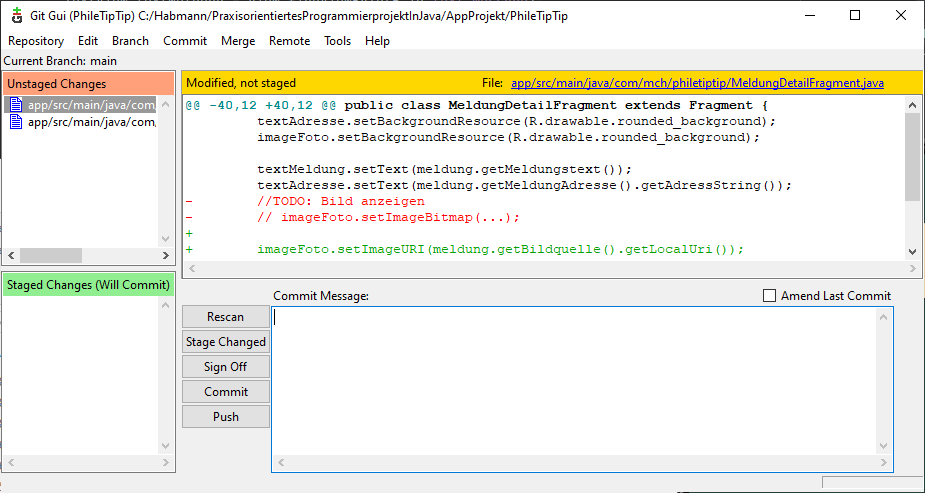
\includegraphics[width=0.6\textwidth]{gitgui}
\caption{Git Gui - Grafisches Tool zur Versionsverwaltung}
\end{figure}

Ein weiterer Vorteil, der sich aus der Verwendung eines Versionierungssystems eröffnet ist die Möglichkeit, einen CI/CD Prozess einzubinden. CI steht in diesem Fall für Continous Integration und bedeutet grob gesagt, dass bei jeder Codeänderung die ein Entwickler in das Versionierungssystem hochläd automatische Prozesse losgetreten werden - in der Regel handelt es sich um einen Build Prozess, der diese Änderungen zusammen mit den aktuellen Änderungen der anderen beteiligten Entwickler zusammen zu einer ausführbaren Anwendung zusammensetzt und in der Regel auch vordefinierte Texts durchführen wird, um zu verhindern, dass fehlerhafte und nicht funktionale Codeänderungen in das Endprodukt einfließen.\\

\begin{figure}[!h]
\centering
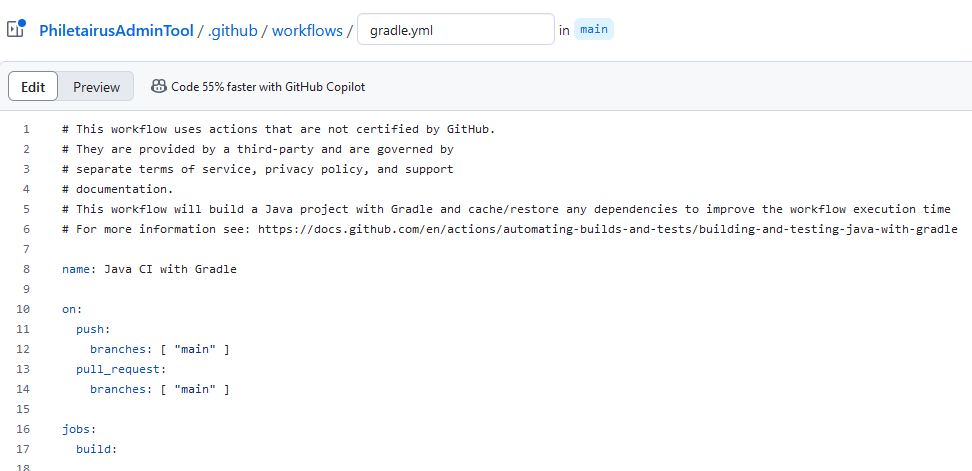
\includegraphics[width=0.6\textwidth]{githubactions}
\caption{Github Actions}
\end{figure}

Das CD kann, je nach gewählten Ansatz entweder für Continous Delivery oder Continous Deployment stehen. In beiden Fällen entsteht nach dem CI Schritt ein ausführbares Produkt, was sowohl im Sinne der Scrum Philosophie als auch des Prince2 Prozesses ist. Der Hauptunterschied besteht darin, dass bei Continous Delivery dieses Zwischenprodukt (welches ein Scrum Inkrement darstellen könnte) zunächst manuell freigegeben werden muss, während es bei Continous Deployment sofort nach bestehen der vordefinierten Tests an die angebundenen Nutzer ausgeliefert wird, wodurch diese ständig Zugriff auf die aktuellste Version haben, wodurch die Feedbackschleife deutlich kürzer gestaltet wird, aber unter Umständen auch Zwischenstände von Funktionen, die noch nicht für den Anwendungstest vorgesehen sind veröffentlicht werden können, in beiden Fällen ist eine durchdachte Kommunikationsstrategie notwendig.

%https://www.rapid7.com/de/cybersecurity-grundlagen/cicd/

\subsubsection{Kommunikation und Projektmanagement}

Ein weiteres Tool auf das sich die Projektbeteiligten geeinigt haben ist Jira \cite{jira} - ein Tool über das Tasks verwaltet werden können und das sich in der agilen Softwareentwicklung bewährt hat. Mit Jira können Tickets zu einzelnen Userstories angelegt, bearbeitet und zugeteilt werden, im Sinne der Selbstorganisation natürlich auch von den Entwicklern selbst. Dieses System erleichtert den Überblick für den Product Owner, schafft Übersicht für die Entwickler und auch für den Lenkungsausschuss sowie Projektmanager. Ein weiterer Nebeneffekt ist, dass durch diese digitale Lösung auf Kanban-Boards oder ähnliches verzichtet werden kann wodurch der Nachhaltigkeitsansatz von Prince2 unterstützt wird.\\

%https://support.atlassian.com/jira-software-cloud/docs/what-is-the-connections-feature/
%https://www.techtarget.com/searchsoftwarequality/definition/software-toolchain
%https://www-atlassian-com.translate.goog/devops/devops-tools/choose-devops-tools?_x_tr_sl=en&_x_tr_tl=de&_x_tr_hl=de&_x_tr_pto=rq

\subsubsection{Frameworks und Bibliotheken}

Frameworks sind Sammlungen von Funktionalitäten, die als Paket in das jeweilige Projekt eingebunden werden, um häufig wiederkehrende Probleme und Herausforderungen zu lösen. Häufig vereinfachen Sie Zugriffe auf andere Bibliotheken, indem sie komplizierte Aufrufe vor dem Entwickler verbergen und eine vereinfachte Implementierung gestatten. Eines dieser Frameworks, welches zum Einsatz kommt ist Jitpack, welches eng mit der Versionsverwaltung über Git zusammenarbeitet.\\

\begin{figure}[!h]
\centering
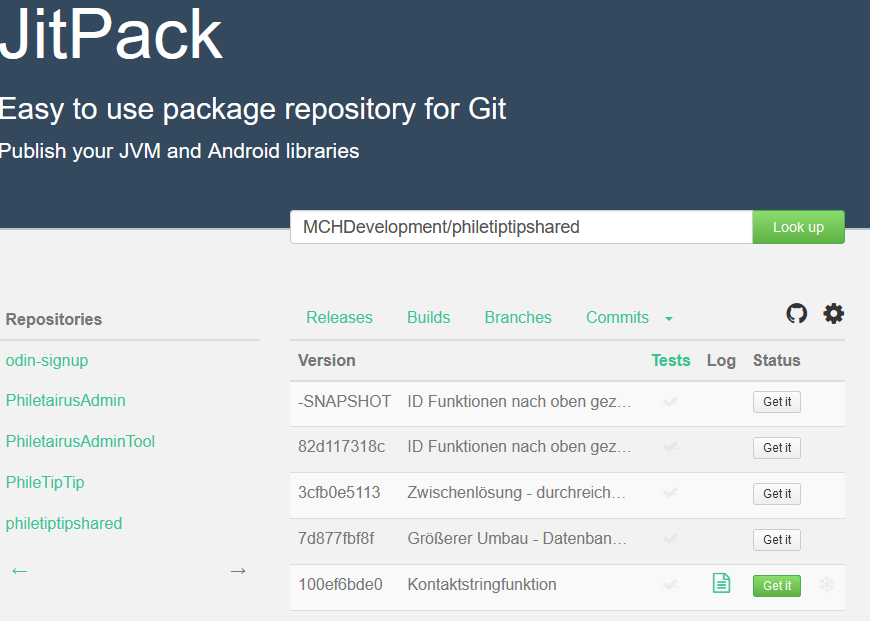
\includegraphics[width=0.6\textwidth]{jitpack}
\caption{Jitpack}
\end{figure}

Jitpack erlaubt es, die in einem Repository (Sammlung der hochgeladenen Dateien) befindlichen Klassen und Funktionen in mehreren Projekten einzubinden, ein entscheidender Vorteil für die zweigeteilte Entwicklung PhileTipTip und Phileteirus Admin Tool, die beide auf gemeinsame Datenklassen (etwa für Mieter, Meldungen und Projekte) zugreifen. So müssen Änderungen nur an einer Stelle vorgenommen werden und es kann nicht zu Inkomptibilitäten oder Redundanzen kommen.\\

Neben diesem Framework werden weitere bewährte Lösungen in der Entwicklungen eingesetzt, wie zum Beispiel JavaFX für die Entwicklung der grafischen Oberfläche des Admintools, welches durch die Gestaltung der GUI mithilfe von FXML in Verbindung mit Controller Klassen ein sehr ähnliches Vorgehen wie Android Studio mit der gestaltung über XML Dateien in Verbindung mit Activities ode Fragmenten zur Kontrolle verfolgt.\\ 

FormsFX und ValidatorFX werden für das Erstellen und Verifizieren von Formularen eingesetzt und das bewährte Spring Framework hilft, eine Struktur bereitzustellen, die modernen Ansprüchen gerecht wird und spätere Anbindungen an weitere Dienste und Erweiterungen erleichtert.\\